% --------------------------------------------------------------
% This is all preamble stuff that you don't have to worry about.
% Head down to where it says "Start here"
% --------------------------------------------------------------
 
\documentclass[12pt]{article}
 
\usepackage[margin=1in]{geometry} 
\usepackage{amsmath,amsthm,amssymb}
\usepackage{mathtools}
\usepackage{enumitem}
\usepackage{graphicx}
\usepackage{listings}
\usepackage{courier}
\usepackage{subcaption}
\usepackage{tikz}
\usepackage{multirow}


\usepackage{algorithm}
\usepackage[noend]{algpseudocode}


\algrenewcommand{\algorithmicreturn}{\State \textbf{return}}

\newcommand{\N}{\mathbb{N}}
\newcommand{\R}{\mathbb{R}}
\newcommand{\LL}{\mathcal{L}}
\newcommand{\LD}{\mathcal{L}_\mathcal{D}}
\newcommand{\LW}{\mathcal{L}_\mathcal{W}}
\newcommand{\norm}[1]{\left\lVert#1\right\rVert}

\lstset{basicstyle=\footnotesize\ttfamily,breaklines=true}
\usepackage{minted}
 

\newcommand{\irow}[1]{% inline row vector
  \begin{smallmatrix}(#1)\end{smallmatrix}%
}

\newcommand{\parder}[2] {
  \frac{\partial{#1} }{\partial{#2}}
}

\setitemize{itemsep=2pt,topsep=4pt,parsep=2pt,partopsep=2pt}
\setenumerate{itemsep=2pt,topsep=4pt,parsep=2pt,partopsep=2pt}

\newenvironment{problem}[2][Problem]{\begin{trivlist}
\item[\hskip \labelsep {\bfseries #1}\hskip \labelsep {\bfseries #2.}]}{\end{trivlist}}
\newenvironment{solution}[1][Solution]{\begin{trivlist}
\item[\hskip \labelsep {\bfseries #1.}]}{\end{trivlist}}


\begin{document}

% --------------------------------------------------------------
%                         Start here
% --------------------------------------------------------------
 
\title{ECE1513 Winter 2019 Assignment 3}

\maketitle

\section{K-means}

\subsection{Learning K-means}

1. We implemented K-Means by minimizing loss function $\mathcal{L}(\mu)$ with AdamOptimizer. The training process early stopped at epoch 541 since the loss cannot be further minimizd. The train loss and clustering result are shown in Figure \ref{fig:a3-1.1-1}.

\begin{figure}[!htb]
\centering
\begin{subfigure}{.5\textwidth}
  \centering
  \includegraphics[width=\linewidth]{images/a3/1.1-1/loss-1.png}
  \caption{Training loss}
\end{subfigure}%
\begin{subfigure}{.5\textwidth}
  \centering
  \includegraphics[width=\linewidth]{images/a3/1.1-1/train-cluster-1.png}
  \caption{Clustering(K=3)}
\end{subfigure}
\caption{K-means clustering with K=3}
\label{fig:a3-1.1-1}
\end{figure}

2. We ran the algorithm with $K = 1,2,3,4,5$ and computed the percentage of the data points belonging to each cluster, as in Table \ref{table:a3-1.1-2}. We also plotted the clustering results in Figure \ref{fig:a3-1.1-2}, to get an intuitive understanding. From the clustering result, we consider $K = 2$ is the best clustering. The reasons are:

\begin{itemize}
    \item The histogram in Figure \ref{fig:a3-1.1-2-hist} shows that the data has two clusters.
    \item From the percentage data and plots, we can see that for $K=2$, data points are roughly divided evenly, and the clustering fits the distribution best. Thus $K=2$ is the best clustering.
    \item For $K=3,4,5$, the 2D plots do not match the actual clustering and the percentage of each clusters are not distributed evenly. These show that $K=3,4,5$ are not good choices. 
\end{itemize}

\begin{table}[!htb]
\centering
\begin{tabular}{|r|r|r|r|r|r|}
\hline
\multicolumn{1}{|c|}{\multirow{2}{*}{K}} & \multicolumn{5}{c|}{Cluster \%} \\ \cline{2-6} 
\multicolumn{1}{|c|}{} & \multicolumn{1}{c|}{0} & \multicolumn{1}{c|}{1} & \multicolumn{1}{c|}{2} & \multicolumn{1}{c|}{3} & \multicolumn{1}{c|}{4} \\ \hline
1 & 100\% &  &  &  &  \\ \hline
2 & 49.5\% & 50.5\% &  &  &  \\ \hline
3 & 23.81\% & 37.97\% & 38.22\% &  &  \\ \hline
4 & 12.03\% & 37.31\% & 37.14\% & 13.52\% &  \\ \hline
5 & 8.57\% & 36.37\% & 7.46\% & 11.71\% & 35.89\% \\ \hline
\end{tabular}
\caption{Percentage of the data points belonging to each clusters, K=1,2,3,4,5}.
\label{table:a3-1.1-2}
\end{table}


\begin{figure}[!htb]
\centering
\begin{subfigure}{.33\linewidth}
  \centering
  \includegraphics[width=\linewidth]{images/a3/1.1-2/train-cluster-1.png}
\end{subfigure}%
\begin{subfigure}{.33\linewidth}
  \centering
  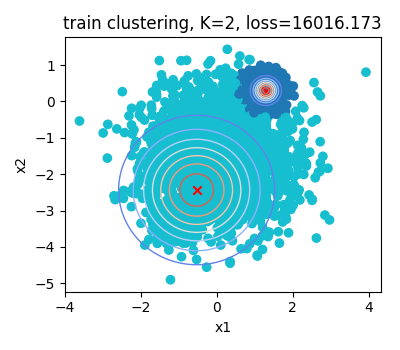
\includegraphics[width=\linewidth]{images/a3/1.1-2/train-cluster-2.png}
\end{subfigure}
\begin{subfigure}{.33\linewidth}
  \centering
  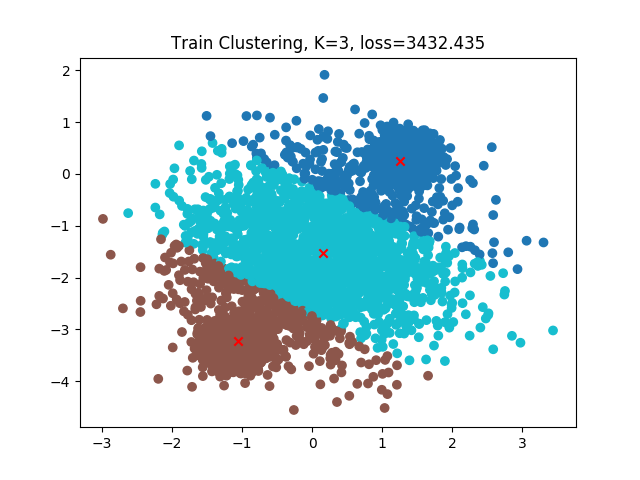
\includegraphics[width=\linewidth]{images/a3/1.1-2/train-cluster-3.png}
\end{subfigure}
\begin{subfigure}{.33\linewidth}
  \centering
  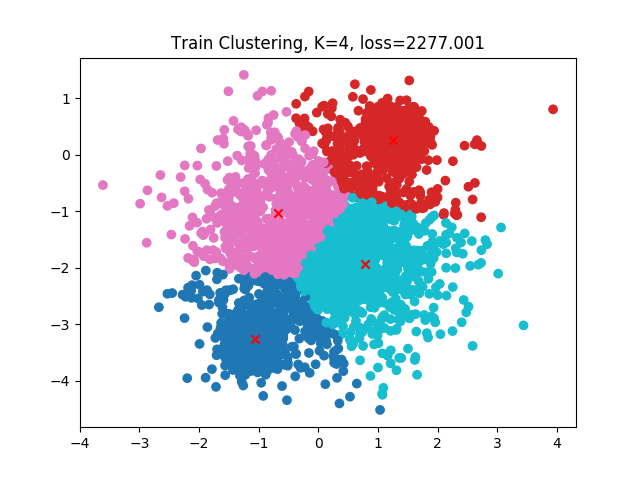
\includegraphics[width=\linewidth]{images/a3/1.1-2/train-cluster-4.png}
\end{subfigure}
\begin{subfigure}{.33\linewidth}
  \centering
  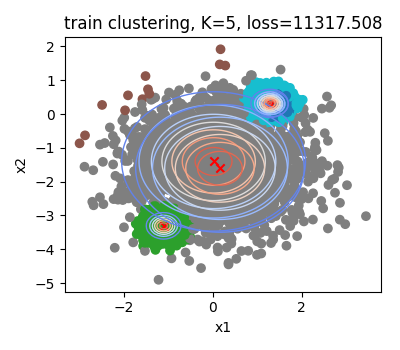
\includegraphics[width=\linewidth]{images/a3/1.1-2/train-cluster-5.png}
\end{subfigure}
\caption{K-means clustering with K=1,2,3,4,5.  Red crosses show the positions of clustering centers.}
\label{fig:a3-1.1-2}
\end{figure}


\begin{figure}[!htb]
\centering
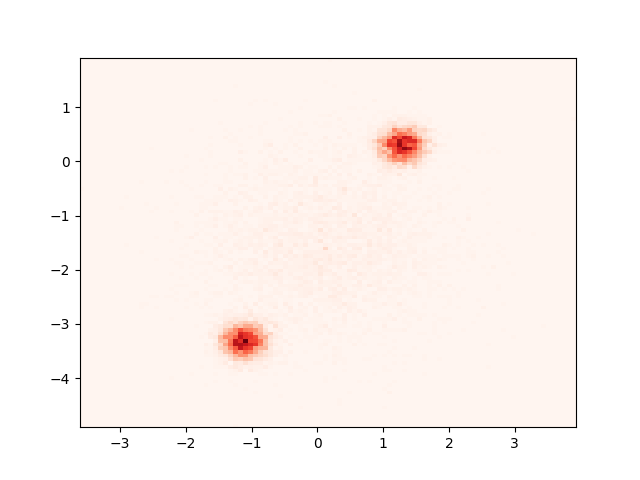
\includegraphics[width=.8\textwidth]{images/a3/1.1-2/data-hist2d.png}
\caption{2D histogram of the training set.}
\label{fig:a3-1.1-2-hist}
\end{figure}

3. We used 1/3 as validation set and trained models on $K=1,2,3,4,5$. Since the loss function $\mathcal{L}(\mu) = \sum_{n=1}^N \min_{k=1}^K \lVert \mathbf{x}_n - \mathbf{\mu}_k \rVert _2^2$ is related to number of data points, the training loss is expected to be two times greater than validation loss. Thus, we compute the ratio of $2 \mathcal{L}_{valid} / \mathcal{L}_{train}$ as the metric of performance. The result is shown in Table \ref{table:a3-1.1-3}.

From Table \ref{table:a3-1.1-3} we can see that $K=2$ has the least valid/train ratio, thus $K=2$ is the best number of clusters.

\begin{table}[!htb]
\centering
\begin{tabular}{r|r|r|r}
\hline
 K & $\mathcal{L}_{train}$ & $\mathcal{L}_{valid}$ & $2 \times \mathcal{L}_{valid} / \mathcal{L}_{train}$ \\ \hline
1 & 25655.162 & 12800.023 & 0.99785 \\
2 & 6231.329 & 2973.207 & 0.95428 \\
3 & 3369.564 & 1746.5096 & 1.03664 \\
4 & 2253.9624 & 1121.8652 & 0.99546 \\
5 & 1866.385 & 1005.4237 & 1.07740 \\ \hline
\end{tabular}
\caption{Training loss vs. Validation loss}
\label{table:a3-1.1-3}
\end{table}

\section{Mixtures of Gaussians}

\subsection{The Gaussian cluster mode}

1. First we compute the log probability density function for cluster $k$.
\begin{align*}
\log\mathcal{N}(\mathbf{x}; \mu_j, \Sigma_j) &= \log\Big(\frac{1}{(2\pi)^{d/2} \sqrt{|\Sigma|}}
    \exp\big(-\frac{1}{2}(\mathbf{x} - \mu)^\intercal \Sigma_j^{-1} (\mathbf{x} - \mu)\big)\Big) \\
&= -0.5d\log(2\pi) -0.5\log|\Sigma| -0.5 (\mathbf{x} - \mu)^\intercal \Sigma_j^{-1} (\mathbf{x} - \mu) \\
&= -0.5 \big( d\log(2\pi) + \log|\Sigma| + (\mathbf{x} - \mu)^\intercal \Sigma_j^{-1} (\mathbf{x} - \mu) \big).
\end{align*}

Given that for the multivariate Gaussian for cluster $k$, different data dimensions are \emph{independent}
and have the \emph{same standard deviation} $\sigma^k$, the covariance for the multivariate Gaussian
is a \emph{diagonal matrix} on $\mathbb{R}^{d\times d}$ with ${\sigma^k}^2$ as its diagonal values. Therefore we have
$$|\Sigma| = ({\sigma^k}^2)^d, \Sigma^{-1} = \mathbf{I} / {\sigma^k}^2.$$

Thus
\begin{align*}
\log\mathcal{N}(\mathbf{x}; \mu_j, \Sigma_j) &=
    -0.5 \big(d\log(2\pi) + \log({\sigma^k}^{2d}) + (\mathbf{x} - \mu)^\intercal \mathbf{I} (\mathbf{x} - \mu) / {\sigma^k}^2 \big) \\
&= -0.5 \big( d\log(2\pi) + d \log({\sigma^k}^2) +
    (\mathbf{x} - \mu)^\intercal (\mathbf{x} - \mu) / {\sigma^k}^2 \big).
\end{align*}

To enable batch computation in Tensorflow, some dimension manipulations are required. See the code snippet below for details.

\begin{minted}
[
frame=lines,
framesep=2mm,
baselinestretch=1.0,
fontsize=\footnotesize,
]{python}
def log_pdf(self, X, Mu, Var):
  """
  Compute the log PDF using multivariate Gaussian distribution.
  :param X: (N x D)
  :param Mu: (K x D)
  :param Var: (K,)
  :return (N x K)
  """
  K, D = Mu.shape.as_list()

  # We need to compute (x - mu)^T @ (x - mu) for all k in K, n in N,
  # where (x - mu) is with shape of (D, 1).
  # Thus the actual multiplication should be done with
  # dist_T(N, K, 1, D) @ dist(N, K, D, 1) => (N, K, 1, 1)
  dist = X[:, None, :, None] - Mu[None, :, :, None]     # (N x K x D x 1)
  dist_T = tf.transpose(dist, (0, 1, 3, 2))             # (N x K x 1 x D)

  return -.5 * (
    D * np.log(2 * np.pi) +
    D * tf.log(Var) +
    tf.reshape(tf.matmul(dist_T, dist), shape=(-1, K)) / Var
  )
\end{minted}


2. First we compute the log probability of the cluster variable $z = k$ given the data vector $\mathbf{x}$:
\begin{align*}
P(z=k|\mathbf{x}) &= P(\mathbf{x}, z=k) \Big/ \sum_{j=1}^K P(\mathbf{x}, z=j) \\
&= P(z=k) P(\mathbf{x} | z=k) \Big/ \sum_{j=1}^K P(z=j) P(\mathbf{x} | z=j),
\end{align*}

where $P(z=j) = \pi_j$ subject to $\pi_j > 0, \sum_{j=1}^K \pi_j = 1$, and
$P(\mathbf{x}|z=j) = \mathcal{N}(\mathbf{x}; \mu_j, {\sigma^j}^2)$. Thus
\begin{align*}
P(z=k|\mathbf{x}) &= \pi_k \mathcal{N}(\mathbf{x}; \mu_k, {\sigma^k}^2) \Big/
    \sum_{j=1}^K \pi_j \mathcal{N}(\mathbf{x}; \mu_j, {\sigma^j}^2), \\
\log P(z=k|\mathbf{x}) &= \log\pi_k + \log \mathcal{N}(\mathbf{x}; \mu_k, {\sigma^k}^2)
    - \log \sum_{j=1}^K \pi_j \mathcal{N}(\mathbf{x}; \mu_j, {\sigma^j}^2).
\end{align*}

Denote $\pi_k = e^{\psi_k} / \sum_k e^{\psi_k}, {\sigma^j}^2 = e^{\phi_k}$, then
\begin{align*}
\log \mathcal{N}(\mathbf{x}; \mu_k, {\sigma^k}^2) &= \text{logpdf}(\mathbf{x}; \mu_k, e^{\phi_k}),\\
\log \pi_k &= \log e^{\psi_k} - \log \sum_k e^{\psi_k} 
    = \psi_k - \text{logsumexp}(\psi), \\
\log \pi &= [\log \pi_1 \cdots \log \pi_K] \\
    &= [\psi_1 - \text{logsumexp}(\psi) \cdots \psi_K - \text{logsumexp}(\psi)] \\
    &= [\psi_1 \cdots \psi_K] - \text{logsumexp}(\psi) \\
    &= \psi - \text{logsumexp}(\psi)
    = \text{logsoftmax}(\psi).
\end{align*}

Thus
\begin{align*}
\log P(z|\mathbf{x}) &= [\log(\pi_1) + \text{logpdf}(\mathbf{x}, \mu_1, e^{\phi_1}) - 
    \text{logsumexp}(\log\pi + \text{logpdf}(\mathbf{x}, \mu, e^{\phi})) \cdots ] \\
    &= \log\pi + \text{logpdf}(\mathbf{x}, \mu, e^\phi) 
    - \text{logsumexp}(\log\pi + \text{logpdf}(\mathbf{x}, \mu, e^{\phi})) \\
    &= \text{logsoftmax}(\psi) + \text{logpdf}(\mathbf{x}, \mu, e^\phi) 
    - \text{logsumexp}(\text{logsoftmax}(\psi) + \text{logpdf}(\mathbf{x}, \mu, e^{\phi})) \\
\end{align*}

You may note that above equation can be further reduced as
$\text{logsoftmax}(\text{logsoftmax}(\psi) + \text{logpdf}(\mathbf{x}, \mu, e^\phi))$. However, when considering multiple data points $\textbf{X} \in \mathbb{R}^{N \times D}$, 
the result of $\text{logsoftmax}(\psi) + \text{logpdf}(\mathbf{x}, \mu, e^\phi) \in \mathbb{R}^{N \times K}$, thus for each single data point, we need the softmax to be computed along the 2nd axis (i.e. the axis with size $K$), not the 1st axis (the axis with size $N$). Since the helper function \texttt{logsoftmax} only computes along the first axis, we cannot use \texttt{logsoftmax} directly here.

\begin{minted}
[
frame=lines,
framesep=2mm,
baselinestretch=1.0,
fontsize=\footnotesize,
]{python}
def log_proba(self, X, Mu, Phi, Psi):
  """Compute the log probability of the cluster variable z given the data vector x.
  :param X: data matrix, (N x D)
  :param Mu: cluster center matrix, (K x D)
  :param Phi: (K,)
  :param Psi: (K,)
  :return (N x K)
  """
  N, D = X.shape
  K = Mu.shape[0]

  logpdf = self.log_pdf(X, Mu, tf.exp(Phi))     # (N x K)
  logw = logsoftmax(Psi)            # (K,)

  logw_pdf = logpdf + logw          # (N x K)
  lse = reduce_logsumexp(logw_pdf, reduction_indices=1, keep_dims=True)   # (N, 1)

  return logw_pdf - lse             # (N x K)
\end{minted}


The reason for using \texttt{logsumexp} instead of \texttt{tf.reduce\_sum} is that,
by subtracting the maximum value from all the components,
\texttt{logsumexp} can prevent data overflow when the vector is extremely large.


\subsection{Learning the MoG}

1. First we compute the equation of loss function, with $\pi_k = e^{\psi_k} / \sum_k e^{\psi_k}$, ${\sigma^j}^2 = e^{\phi_k}$:
\begin{align*}
\mathcal{L}(\mu, \psi, \phi) &= -\log \prod_n \sum_k \pi^k \mathcal{N}(\mathbf{x}_n; \mu^k, {\sigma^k}^2) \\
&= -\sum_n \log \sum_k \pi^k \mathcal{N}(\mathbf{x}_n; \mu^k, {\sigma^k}^2) \\
&= -\sum_n \log \sum_k \exp \big(\log\pi^k + \log \mathcal{N}(\mathbf{x}_n; \mu^k, {\sigma^k}^2) \big) \\
&= -\sum_n \text{logsumexp}\big(\log\pi + \log \mathcal{N}(\mathbf{x}_n; \mu, \sigma^2) \big) \\
&= -\sum_n \text{logsumexp} \big( \text{logsoftmax}(\psi) + \text{logpdf}(\mathbf{x}_n, \mu, e^\phi) \big).
\end{align*}

We implemented the loss function and trained a MoG model with $K=3$. After early stop at epoch 511, the best parameters are:
$$ \mu = \begin{bmatrix*}[r]
-1.1011823 & -3.3061764 \\
1.298578  &  0.3091123 \\
0.10558542 & -1.5281174
\end{bmatrix*}, 
\phi = \begin{bmatrix*}[r]-3.242426  \\ -3.2409697 \\ -0.01329159\end{bmatrix*},
\psi = \begin{bmatrix*}[r]0.13701023 \\ 0.14201044 \\ 0.1449725\end{bmatrix*} $$

The loss plot and clustering are shown in Figure \ref{fig:a3-2.2-1}.
For demonstration purpose we also plot the contour of each Gaussian.

\begin{figure}[!htb]
\centering
\begin{subfigure}{.5\textwidth}
  \centering
  \includegraphics[width=\linewidth]{images/a3/2.2-1/loss-1.png}
  \caption{Training loss}
\end{subfigure}%
\begin{subfigure}{.5\textwidth}
  \centering
  \includegraphics[width=\linewidth]{images/a3/2.2-1/train-cluster-1.png}
  \caption{Clustering(K=3)}
\end{subfigure}
\caption{Mixture of Gaussians clustering with K=3. Red cross shows the clustering center while the contour shows the density of each Gaussian distribution.}
\label{fig:a3-2.2-1}
\end{figure}

\bigskip

2. Table \ref{table:a3-2.2-2} shows the training and validation loss for $K=1,2,3,4,5$. Since the loss function is related with data size, we compute the ratio of validation loss and training loss. The minimum of ratio appears at $K = 3$, indicating that $K=3$ is the best clustering.

The clustering plot of each $K$ value is shown in Figure \ref{fig:a3-2.2-2}.

\begin{table}[!htb]
\centering
\begin{tabular}{r|r|r|r}
\hline
 K & $\mathcal{L}_{train}$ & $\mathcal{L}_{valid}$ & $2 \mathcal{L}_{valid} / \mathcal{L}_{train}$ \\ \hline
1 & 23296.97 & 11619.322 & 0.99750 \\
2 & 16016.173 & 8125.6406 & 1.01468 \\
3 & 11458.64 & 5678.3496 & 0.99110 \\
4 & 11354.237 & 5782.4033 & 1.01855 \\
5 & 11317.508 & 5819.642 & 1.02843 \\
\hline
\end{tabular}
\caption{Training loss vs. Validation loss}
\label{table:a3-2.2-2}
\end{table}

\begin{figure}[!htb]
\centering
\begin{subfigure}{.33\linewidth}
  \centering
  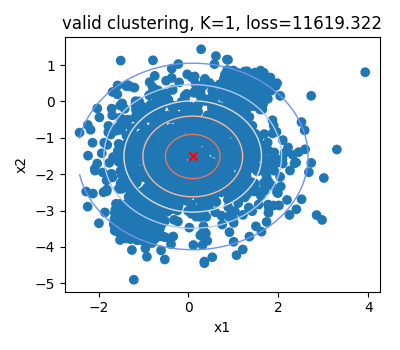
\includegraphics[width=\linewidth]{images/a3/2.2-2/valid-cluster-1.png}
\end{subfigure}%
\begin{subfigure}{.33\linewidth}
  \centering
  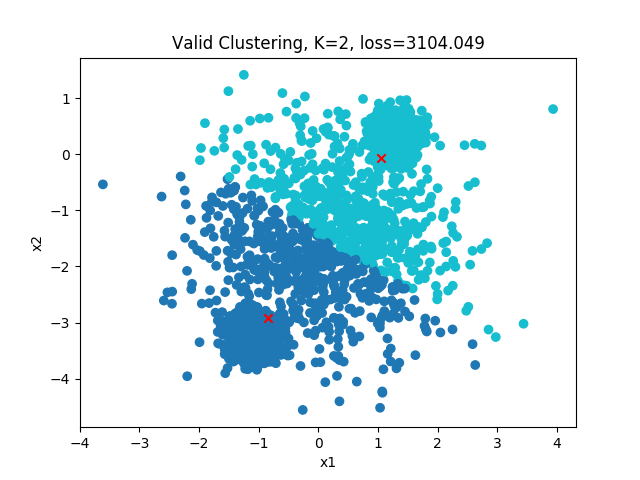
\includegraphics[width=\linewidth]{images/a3/2.2-2/valid-cluster-2.png}
\end{subfigure}
\begin{subfigure}{.33\linewidth}
  \centering
  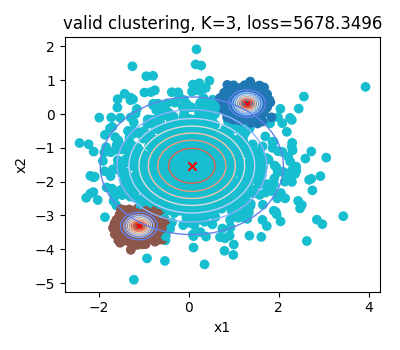
\includegraphics[width=\linewidth]{images/a3/2.2-2/valid-cluster-3.png}
\end{subfigure}
\begin{subfigure}{.33\linewidth}
  \centering
  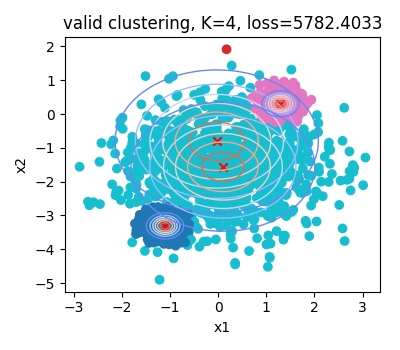
\includegraphics[width=\linewidth]{images/a3/2.2-2/valid-cluster-4.png}
\end{subfigure}
\begin{subfigure}{.33\linewidth}
  \centering
  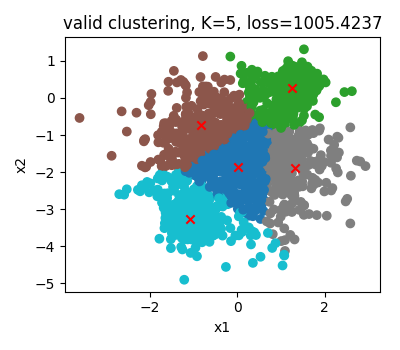
\includegraphics[width=\linewidth]{images/a3/2.2-2/valid-cluster-5.png}
\end{subfigure}
\caption{Mixture of Gaussians clustering with K=1,2,3,4,5}
\label{fig:a3-2.2-2}
\end{figure}

\bigskip

3. We run both K-means and MoG on dataset \emph{data100D.npy} and plot the clustering in Figure \ref{fig:a3-2.2-3-kmeans} and Figure \ref{fig:a3-2.2-3-mog}.
The 100-D input data is reduced to 2-D with PCA, while PC1 and PC2 account for 24\% and 21\% of the variation respectively. Intuitively $K=10$ is the best clustering for both algorithms, however we need a quantitative metric to evaluate their performance. 
We choose \emph{silhouette score} as the metric of clustering. \emph{Silhouette score} is a metric of how similar a data point is similar to its own cluster than to other clusters. Given point $\mathbf{x}$, denote the mean intra-cluster distance as $a$ and the mean nearest-cluster distance as $b$, then the silhouette score is $(b - a) / \max(a, b)$. 

Both K-means and MoG cannot guarantee global minima when using gradient descent as optimization. Thus we run the clustering 10 times for each algorithm and compute the average silhouette score with \texttt{sklearn.metric.silhouette\_score}. The result score is shown in Table \ref{table:a3-2.2.3-silhouette} and Figure \ref{fig:a3-2.2-3-silhouette}.

The silhouette scores show that for K-means and MoG, the best clusterings are $K=10$ and $K=15$ respectively.


\begin{table}[!htb]
\centering
\begin{tabular}{r|r|r|r|r}
\hline
 k &  K-means mean & K-means stddev & MoG mean & MoG stddev \\
\hline
 5 &     0.517469 &    0.043120 &  0.380841 &  0.088725 \\
10 &     \underline{0.528677} &    0.100117 &  0.530042 &  0.051024 \\
15 &     0.489333 &    0.083503 &  \underline{0.552551} &  0.083270 \\
20 &     0.451246 &    0.093502 &  0.536086 &  0.065657 \\
30 &     0.402536 &    0.061891 &  0.469634 &  0.077099 \\
\hline
\end{tabular}
\caption{Mean and standard deviation of silhouette scores for 10 runs of K-means and MoG. The best clusterings are underlined.}
\label{table:a3-2.2.3-silhouette}
\end{table}


\begin{figure}[!htb]
\centering
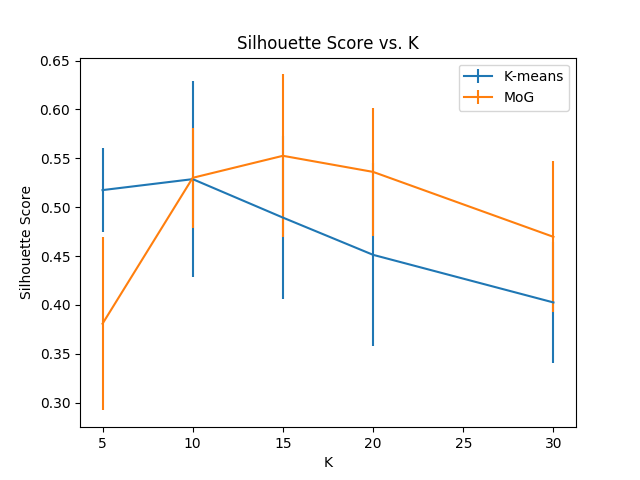
\includegraphics[width=.6\linewidth]{images/a3/2.2-3/silhouette.png}
\caption{Silhouette score for K=5,10,15,20,30}
\label{fig:a3-2.2-3-silhouette}
\end{figure}

\begin{figure}[!htb]
\centering
\begin{subfigure}{.33\linewidth}
  \centering
  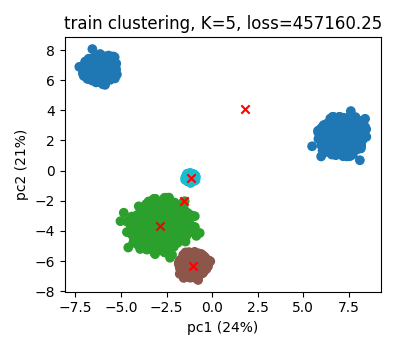
\includegraphics[width=\linewidth]{images/a3/2.2-3/train-cluster-kmeans-5.png}
\end{subfigure}%
\begin{subfigure}{.33\linewidth}
  \centering
  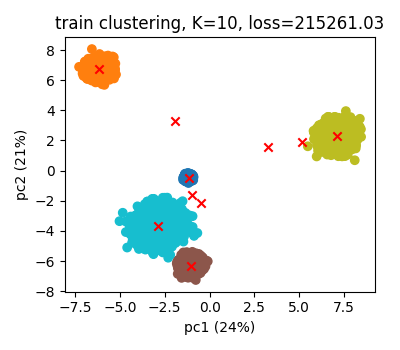
\includegraphics[width=\linewidth]{images/a3/2.2-3/train-cluster-kmeans-10.png}
\end{subfigure}
\begin{subfigure}{.33\linewidth}
  \centering
  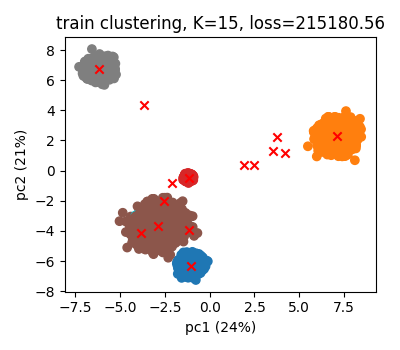
\includegraphics[width=\linewidth]{images/a3/2.2-3/train-cluster-kmeans-15.png}
\end{subfigure}
\begin{subfigure}{.33\linewidth}
  \centering
  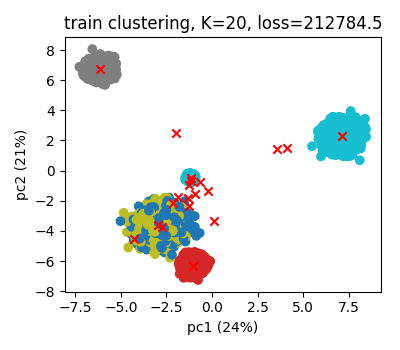
\includegraphics[width=\linewidth]{images/a3/2.2-3/train-cluster-kmeans-20.png}
\end{subfigure}
\begin{subfigure}{.33\linewidth}
  \centering
  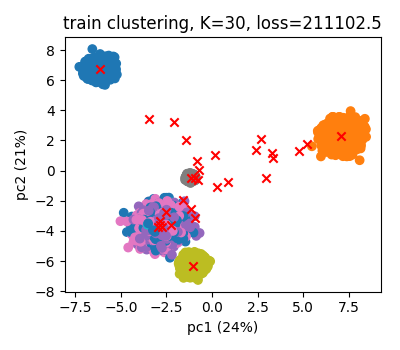
\includegraphics[width=\linewidth]{images/a3/2.2-3/train-cluster-kmeans-30.png}
\end{subfigure}
\caption{K-means clustering with K=1,2,3,4,5 on data100D}
\label{fig:a3-2.2-3-kmeans}
\end{figure}


\begin{figure}[!htb]
\centering
\begin{subfigure}{.33\linewidth}
  \centering
  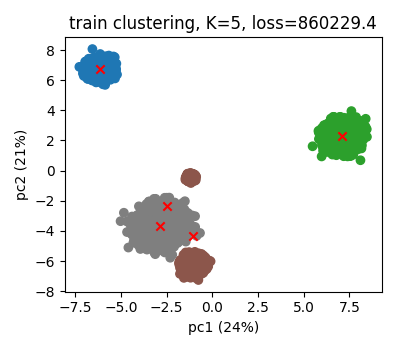
\includegraphics[width=\linewidth]{images/a3/2.2-3/train-cluster-mog-5.png}
\end{subfigure}%
\begin{subfigure}{.33\linewidth}
  \centering
  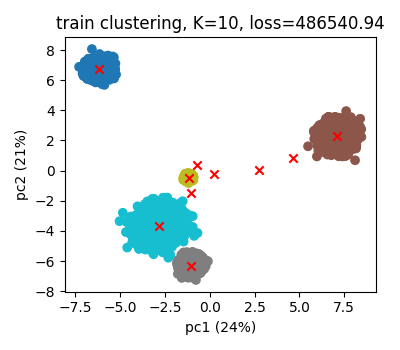
\includegraphics[width=\linewidth]{images/a3/2.2-3/train-cluster-mog-10.png}
\end{subfigure}
\begin{subfigure}{.33\linewidth}
  \centering
  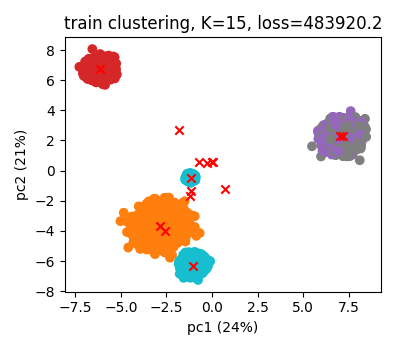
\includegraphics[width=\linewidth]{images/a3/2.2-3/train-cluster-mog-15.png}
\end{subfigure}
\begin{subfigure}{.33\linewidth}
  \centering
  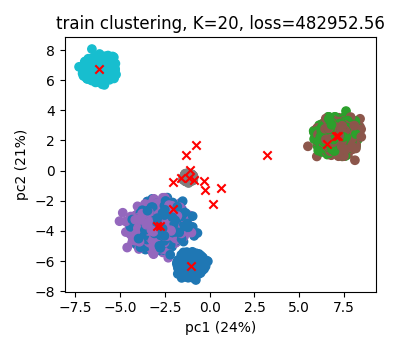
\includegraphics[width=\linewidth]{images/a3/2.2-3/train-cluster-mog-20.png}
\end{subfigure}
\begin{subfigure}{.33\linewidth}
  \centering
  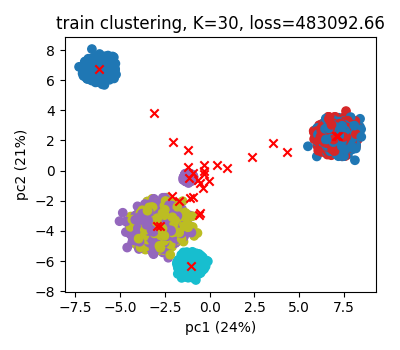
\includegraphics[width=\linewidth]{images/a3/2.2-3/train-cluster-mog-30.png}
\end{subfigure}
\caption{MoG clustering with K=1,2,3,4,5 on data100D}
\label{fig:a3-2.2-3-mog}
\end{figure}


\newpage

\end{document}
